\documentclass{article}\usepackage[]{graphicx}\usepackage[]{color}
% maxwidth is the original width if it is less than linewidth
% otherwise use linewidth (to make sure the graphics do not exceed the margin)
\makeatletter
\def\maxwidth{ %
  \ifdim\Gin@nat@width>\linewidth
    \linewidth
  \else
    \Gin@nat@width
  \fi
}
\makeatother

\definecolor{fgcolor}{rgb}{0.345, 0.345, 0.345}
\newcommand{\hlnum}[1]{\textcolor[rgb]{0.686,0.059,0.569}{#1}}%
\newcommand{\hlstr}[1]{\textcolor[rgb]{0.192,0.494,0.8}{#1}}%
\newcommand{\hlcom}[1]{\textcolor[rgb]{0.678,0.584,0.686}{\textit{#1}}}%
\newcommand{\hlopt}[1]{\textcolor[rgb]{0,0,0}{#1}}%
\newcommand{\hlstd}[1]{\textcolor[rgb]{0.345,0.345,0.345}{#1}}%
\newcommand{\hlkwa}[1]{\textcolor[rgb]{0.161,0.373,0.58}{\textbf{#1}}}%
\newcommand{\hlkwb}[1]{\textcolor[rgb]{0.69,0.353,0.396}{#1}}%
\newcommand{\hlkwc}[1]{\textcolor[rgb]{0.333,0.667,0.333}{#1}}%
\newcommand{\hlkwd}[1]{\textcolor[rgb]{0.737,0.353,0.396}{\textbf{#1}}}%
\let\hlipl\hlkwb

\usepackage{framed}
\makeatletter
\newenvironment{kframe}{%
 \def\at@end@of@kframe{}%
 \ifinner\ifhmode%
  \def\at@end@of@kframe{\end{minipage}}%
  \begin{minipage}{\columnwidth}%
 \fi\fi%
 \def\FrameCommand##1{\hskip\@totalleftmargin \hskip-\fboxsep
 \colorbox{shadecolor}{##1}\hskip-\fboxsep
     % There is no \\@totalrightmargin, so:
     \hskip-\linewidth \hskip-\@totalleftmargin \hskip\columnwidth}%
 \MakeFramed {\advance\hsize-\width
   \@totalleftmargin\z@ \linewidth\hsize
   \@setminipage}}%
 {\par\unskip\endMakeFramed%
 \at@end@of@kframe}
\makeatother

\definecolor{shadecolor}{rgb}{.97, .97, .97}
\definecolor{messagecolor}{rgb}{0, 0, 0}
\definecolor{warningcolor}{rgb}{1, 0, 1}
\definecolor{errorcolor}{rgb}{1, 0, 0}
\newenvironment{knitrout}{}{} % an empty environment to be redefined in TeX

\usepackage{alltt}
\usepackage[sc]{mathpazo}
\renewcommand{\sfdefault}{lmss}
\renewcommand{\ttdefault}{lmtt}
\usepackage[T1]{fontenc}
\usepackage{geometry}
\geometry{verbose,tmargin=2.5cm,bmargin=2.5cm,lmargin=2.5cm,rmargin=2.5cm}
\setcounter{secnumdepth}{2}
\setcounter{tocdepth}{2}
\usepackage[unicode=true,pdfusetitle,
 bookmarks=true,bookmarksnumbered=true,bookmarksopen=true,bookmarksopenlevel=2,
 breaklinks=false,pdfborder={0 0 1},backref=false,colorlinks=false]
 {hyperref}
\hypersetup{
 pdfstartview={XYZ null null 1}}

\makeatletter
%%%%%%%%%%%%%%%%%%%%%%%%%%%%%% User specified LaTeX commands.
\renewcommand{\textfraction}{0.05}
\renewcommand{\topfraction}{0.8}
\renewcommand{\bottomfraction}{0.8}
\renewcommand{\floatpagefraction}{0.75}

\makeatother
\IfFileExists{upquote.sty}{\usepackage{upquote}}{}
\begin{document}








The results below are generated from an R script.

\begin{knitrout}
\definecolor{shadecolor}{rgb}{0.969, 0.969, 0.969}\color{fgcolor}\begin{kframe}
\begin{alltt}
\hlkwd{library}\hlstd{(haven)}
\hlkwd{library}\hlstd{(tidyverse)}
\end{alltt}


{\ttfamily\noindent\itshape\color{messagecolor}{\#\# -- Attaching packages ------------------------------------------------- tidyverse 1.3.0 --}}

{\ttfamily\noindent\itshape\color{messagecolor}{\#\# v ggplot2 3.3.2\ \ \ \  v purrr\ \  0.3.4\\\#\# v tibble\ \ 3.0.4\ \ \ \  v dplyr\ \  1.0.2\\\#\# v tidyr\ \  1.1.2\ \ \ \  v stringr 1.4.0\\\#\# v readr\ \  1.4.0\ \ \ \  v forcats 0.5.0}}

{\ttfamily\noindent\itshape\color{messagecolor}{\#\# -- Conflicts ---------------------------------------------------- tidyverse\_conflicts() --\\\#\# x dplyr::filter() masks stats::filter()\\\#\# x dplyr::lag()\ \ \ \ masks stats::lag()}}\begin{alltt}
\hlkwd{library}\hlstd{(randomForest)}
\end{alltt}


{\ttfamily\noindent\itshape\color{messagecolor}{\#\# randomForest 4.6-14}}

{\ttfamily\noindent\itshape\color{messagecolor}{\#\# Type rfNews() to see new features/changes/bug fixes.}}

{\ttfamily\noindent\itshape\color{messagecolor}{\#\# \\\#\# Attaching package: 'randomForest'}}

{\ttfamily\noindent\itshape\color{messagecolor}{\#\# The following object is masked from 'package:dplyr':\\\#\# \\\#\#\ \ \ \  combine}}

{\ttfamily\noindent\itshape\color{messagecolor}{\#\# The following object is masked from 'package:ggplot2':\\\#\# \\\#\#\ \ \ \  margin}}\begin{alltt}
\hlkwd{library}\hlstd{(ggthemes)}

\hlcom{# dataset based on:}
\hlcom{# Generating Skilled Self-Employment in Developing Countries: Experimental Evidence }
\hlcom{# from Uganda (Blattman et al, 2014)}
\hlcom{# outcome of interest is profit in last four weeks capped at 99th percentile; }
\hlcom{# treatment is randomised assignment to the Program (intent to treat)}
\hlcom{# method is based on:}
\hlcom{# Generic Machine Learning Inference on Heterogenous Treatment Effects in Randomized }
\hlcom{# Experiments (Chernozhukov et al, 2017)}
\hlcom{# Note: This is merely preliminary EDA and will be refined once more of the data is }
\hlcom{# understood}
\hlcom{# Final code will be run with neural nets and other forest based methods to derive }
\hlcom{# Best Linear Predictor}

\hlcom{#some data cleaning}

\hlstd{x}\hlkwb{<-}\hlkwd{cbind}\hlstd{(}\hlkwd{read_dta}\hlstd{(}\hlstr{'https://www.dropbox.com/s/yxgigmtcrut9fii/yop_analysis.dta?dl=1'}\hlstd{)} \hlopt
  \hlkwd{filter}\hlstd{(e1}\hlopt{==}\hlnum{1}\hlstd{)} \hlopt  \hlcom{#filter results only from endline survey1}
  \hlkwd{select}\hlstd{(assigned,loan_100k,loan_1mil,grantsize_pp_US_est3,}
         \hlstd{risk_aversion,female,urban,age,live_together,}
                       \hlstd{literate,voc_training,inschool,aggression_n,}
                       \hlstd{violence_others,education,wealthindex,}
                       \hlstd{risk_aversion,profits4w_real_p99_e),}
  \hlkwd{read_dta}\hlstd{(}\hlstr{'https://www.dropbox.com/s/fa7lh4qe8nszxdb/yop_fulldata.dta?dl=1'}\hlstd{)} \hlopt
  \hlkwd{filter}\hlstd{(e1}\hlopt{==}\hlnum{1}\hlstd{)} \hlopt
  \hlkwd{select}\hlstd{(hhsize,acres,credit_access))}

\hlcom{#compute proportion of all NA values}
\hlkwd{sum}\hlstd{(x}\hlopt\hlkwd{is.na}\hlstd{())}\hlopt{/}\hlstd{(}\hlkwd{ncol}\hlstd{(x)}\hlopt{*}\hlkwd{nrow}\hlstd{(x))}
\end{alltt}
\begin{verbatim}
## [1] 0.0213672
\end{verbatim}
\begin{alltt}
\hlcom{#compute proportion of missing outcome values}
\hlkwd{sum}\hlstd{(x}\hlopt{$}\hlstd{profits4w_real_p99_e}\hlopt\hlkwd{is.na}\hlstd{())}\hlopt{/}\hlkwd{nrow}\hlstd{(x)}
\end{alltt}
\begin{verbatim}
## [1] 0.2510273
\end{verbatim}
\begin{alltt}
\hlcom{#eliminate NA values (assume missingness is random)}
\hlcom{#df<-x[which(complete.cases(x)),]}

\hlcom{#impute outcome values using median (assume missingness is non random)}
\hlstd{df}\hlkwb{<-}\hlstd{x} \hlopt \hlkwd{mutate}\hlstd{(}\hlkwc{profits4w_real_p99_e}\hlstd{=}\hlkwd{ifelse}\hlstd{(}\hlkwd{is.na}\hlstd{(profits4w_real_p99_e),}
                                             \hlkwd{median}\hlstd{(x}\hlopt{$}\hlstd{profits4w_real_p99_e,}\hlkwc{na.rm} \hlstd{= T),}
                                             \hlstd{profits4w_real_p99_e))}

\hlcom{#impute NA values for other vars}
\hlstd{df}\hlkwb{<-}\hlkwd{rfImpute}\hlstd{(profits4w_real_p99_e}\hlopt{~}\hlstd{.,df,}\hlkwc{ntree}\hlstd{=}\hlnum{500}\hlstd{,}\hlkwc{iter}\hlstd{=}\hlnum{6}\hlstd{)}
\end{alltt}
\begin{verbatim}
##      |      Out-of-bag   |
## Tree |      MSE  %Var(y) |
##  500 |     5289    97.51 |
##      |      Out-of-bag   |
## Tree |      MSE  %Var(y) |
##  500 |     5300    97.70 |
##      |      Out-of-bag   |
## Tree |      MSE  %Var(y) |
##  500 |     5268    97.11 |
##      |      Out-of-bag   |
## Tree |      MSE  %Var(y) |
##  500 |     5270    97.15 |
##      |      Out-of-bag   |
## Tree |      MSE  %Var(y) |
##  500 |     5294    97.59 |
##      |      Out-of-bag   |
## Tree |      MSE  %Var(y) |
##  500 |     5283    97.39 |
\end{verbatim}
\begin{alltt}
\hlcom{# create empty dataframes to store values}
\hlstd{n_split}\hlkwb{<-}\hlnum{100}
\hlstd{n_group}\hlkwb{<-}\hlnum{5}
\hlstd{blp_coef}\hlkwb{<-}\hlkwd{data.frame}\hlstd{(}\hlkwc{B0}\hlstd{=}\hlnum{1}\hlopt{:}\hlstd{n_split,}\hlkwc{SE_B0}\hlstd{=}\hlnum{1}\hlopt{:}\hlstd{n_split,}
                     \hlkwc{P_value_B0}\hlstd{=}\hlnum{1}\hlopt{:}\hlstd{n_split,}
                     \hlkwc{B1}\hlstd{=}\hlnum{1}\hlopt{:}\hlstd{n_split,}\hlkwc{SE_B1}\hlstd{=}\hlnum{1}\hlopt{:}\hlstd{n_split,}
                     \hlkwc{P_value_B1}\hlstd{=}\hlnum{1}\hlopt{:}\hlstd{n_split)}

\hlstd{gate_coef}\hlkwb{<-}\hlkwd{matrix}\hlstd{(}\hlkwc{ncol} \hlstd{= n_group}\hlopt{*}\hlnum{2}\hlstd{,}\hlkwc{nrow} \hlstd{= n_split)} \hlopt \hlkwd{as.data.frame}\hlstd{()}
\hlkwd{colnames}\hlstd{(gate_coef)}\hlkwb{<-}\hlkwd{paste}\hlstd{(}\hlkwd{c}\hlstd{(}\hlstr{"G"}\hlstd{,}\hlstr{'SE_G'}\hlstd{),} \hlkwd{rep}\hlstd{(}\hlnum{1}\hlopt{:}\hlstd{n_group,} \hlkwc{each}\hlstd{=}\hlnum{2}\hlstd{),} \hlkwc{sep} \hlstd{=} \hlstr{""}\hlstd{)}

\hlcom{#f<-which(sapply(df, class) == "factor") }
\hlcom{#mcol<-ncol(df[,-f])}
\hlstd{mcol}\hlkwb{<-}\hlkwd{ncol}\hlstd{(df)}
\hlstd{gate_mean}\hlkwb{<-}\hlkwd{matrix}\hlstd{(}\hlkwc{ncol} \hlstd{= mcol}\hlopt{*}\hlstd{n_group,}\hlkwc{nrow} \hlstd{= n_split)}
\hlkwd{colnames}\hlstd{(gate_mean)}\hlkwb{<-}\hlkwd{rep}\hlstd{(}\hlkwd{colnames}\hlstd{(df[,]),n_group)}

\hlcom{#split data}
\hlkwd{set.seed}\hlstd{(}\hlnum{55}\hlstd{,}\hlkwc{sample.kind} \hlstd{=} \hlstr{'Rounding'}\hlstd{)}
\end{alltt}


{\ttfamily\noindent\color{warningcolor}{\#\# Warning in set.seed(55, sample.kind = "{}Rounding"{}): non-uniform 'Rounding' sampler used}}\begin{alltt}
\hlkwa{for}\hlstd{(i} \hlkwa{in} \hlnum{1}\hlopt{:}\hlstd{n_split)\{}

  \hlcom{#randomly split data into main and auxiliary }
  \hlstd{random}\hlkwb{<-}\hlkwd{runif}\hlstd{(}\hlkwd{nrow}\hlstd{(df))}
  \hlstd{main_ind}\hlkwb{<-}\hlkwd{which}\hlstd{(random}\hlopt{>}\hlnum{0.5}\hlstd{)}
  \hlstd{aux_ind}\hlkwb{<-}\hlkwd{which}\hlstd{(random}\hlopt{<}\hlnum{0.5}\hlstd{)}
  \hlstd{aux_df}\hlkwb{<-}\hlstd{df[aux_ind,]}

  \hlcom{# train data on auxiliary sample}
  \hlstd{rftreat}\hlkwb{<-}\hlkwd{randomForest}\hlstd{(profits4w_real_p99_e}\hlopt{~}\hlstd{.,} \hlkwc{data} \hlstd{= (aux_df}\hlopt\hlkwd{filter}\hlstd{(assigned}\hlopt{==}\hlnum{1}\hlstd{)),}
                        \hlkwc{ntree}\hlstd{=}\hlnum{500}\hlstd{,}\hlkwc{nodesize}\hlstd{=}\hlnum{5}\hlstd{)}
  \hlstd{rfbase}\hlkwb{<-}\hlkwd{randomForest}\hlstd{(profits4w_real_p99_e}\hlopt{~}\hlstd{.,} \hlkwc{data} \hlstd{= (aux_df}\hlopt\hlkwd{filter}\hlstd{(assigned}\hlopt{==}\hlnum{0}\hlstd{)),}
                       \hlkwc{ntree}\hlstd{=}\hlnum{500}\hlstd{,}\hlkwc{nodesize}\hlstd{=}\hlnum{5}\hlstd{)}

  \hlcom{# predict baseline and treatment outcomes}
  \hlstd{B}\hlkwb{<-}\hlkwd{predict}\hlstd{(rfbase,df)}
  \hlstd{treat}\hlkwb{<-}\hlkwd{predict}\hlstd{(rftreat,df)}

  \hlcom{# specifying regression variables}
  \hlstd{S}\hlkwb{<-}\hlstd{treat}\hlopt{-}\hlstd{B} \hlcom{#CATE}
  \hlstd{ES}\hlkwb{<-}\hlkwd{mean}\hlstd{(S)}
  \hlstd{p}\hlkwb{<-}\hlkwd{mean}\hlstd{(df}\hlopt{$}\hlstd{assigned)} \hlcom{#take mean as propensity score}
  \hlstd{x}\hlkwb{<-}\hlstd{S}\hlopt{-}\hlstd{ES} \hlcom{#excess CATE}
  \hlstd{w}\hlkwb{<-}\hlstd{df}\hlopt{$}\hlstd{assigned}\hlopt{-}\hlstd{p} \hlcom{#weighted treatment var}

  \hlcom{#derive Best Linear Predictor from main sample}
  \hlstd{blp}\hlkwb{<-}\hlkwd{lm}\hlstd{(profits4w_real_p99_e}\hlopt{~}\hlstd{B}\hlopt{+}\hlstd{w}\hlopt{+}\hlkwd{I}\hlstd{((w}\hlopt{*}\hlstd{x)),}\hlkwc{data}\hlstd{=}\hlkwd{cbind}\hlstd{(df,B,S,x,w)[main_ind,])}
  \hlstd{blp_coef[i,]}\hlkwb{<-}\hlkwd{c}\hlstd{(blp}\hlopt{$}\hlstd{coefficients[}\hlnum{3}\hlstd{],}\hlkwd{summary}\hlstd{(blp)}\hlopt{$}\hlstd{coefficients[}\hlnum{3}\hlopt{:}\hlnum{4}\hlstd{,}\hlkwd{c}\hlstd{(}\hlnum{2}\hlstd{,}\hlnum{4}\hlstd{)][}\hlnum{1}\hlstd{,],}
                  \hlstd{blp}\hlopt{$}\hlstd{coefficients[}\hlnum{4}\hlstd{],}\hlkwd{summary}\hlstd{(blp)}\hlopt{$}\hlstd{coefficients[}\hlnum{3}\hlopt{:}\hlnum{4}\hlstd{,}\hlkwd{c}\hlstd{(}\hlnum{2}\hlstd{,}\hlnum{4}\hlstd{)][}\hlnum{2}\hlstd{,])}


  \hlcom{#Group Average Treatment Effect}
  \hlstd{qt}\hlkwb{<-}\hlkwd{quantile}\hlstd{(S,}\hlkwd{seq}\hlstd{(}\hlnum{0}\hlstd{,}\hlnum{1}\hlstd{,}\hlkwc{length.out} \hlstd{= n_group}\hlopt{+}\hlnum{1}\hlstd{))}

  \hlkwa{for}\hlstd{(k} \hlkwa{in} \hlnum{1}\hlopt{:}\hlstd{n_group)\{}
    \hlstd{G}\hlkwb{<-}\hlkwd{ifelse}\hlstd{(S}\hlopt{>}\hlstd{qt[k]} \hlopt{&} \hlstd{S}\hlopt{<}\hlstd{qt[k}\hlopt{+}\hlnum{1}\hlstd{],}\hlnum{1}\hlstd{,}\hlnum{0}\hlstd{)}
    \hlstd{gate}\hlkwb{<-}\hlkwd{lm}\hlstd{(profits4w_real_p99_e}\hlopt{~}\hlstd{B}\hlopt{+}\hlkwd{I}\hlstd{(w}\hlopt{*}\hlstd{G),}\hlkwc{data} \hlstd{=} \hlkwd{cbind}\hlstd{(df,B,S,x,w,G)[main_ind,])}
    \hlstd{gate_coef[i,}\hlkwd{c}\hlstd{((}\hlnum{2}\hlopt{*}\hlstd{k)}\hlopt{-}\hlnum{1}\hlstd{,}\hlnum{2}\hlopt{*}\hlstd{k)]}\hlkwb{<-}\hlkwd{summary}\hlstd{(gate)}\hlopt{$}\hlstd{coefficients[}\hlnum{3}\hlstd{,}\hlkwd{c}\hlstd{(}\hlnum{1}\hlstd{,}\hlnum{2}\hlstd{)]}

    \hlcom{# data preparation for later}
    \hlstd{gate_mean[i,((k}\hlopt{*}\hlstd{mcol)}\hlopt{-}\hlstd{(mcol}\hlopt{-}\hlnum{1}\hlstd{))}\hlopt{:}\hlstd{(k}\hlopt{*}\hlstd{mcol)]}\hlkwb{<-}\hlkwd{apply}\hlstd{(df[}\hlkwd{which}\hlstd{(G}\hlopt{==}\hlnum{1}\hlstd{),],}\hlnum{2}\hlstd{,mean)}
  \hlstd{\}}
\hlstd{\}}

\hlcom{# obtain median values}
\hlcom{# data for each column does not correspond to the same split}
\hlkwd{apply}\hlstd{(blp_coef,}\hlnum{2}\hlstd{,median)} \hlcom{#median for Best Linear Predictor }
\end{alltt}
\begin{verbatim}
##           B0        SE_B0   P_value_B0           B1        SE_B1   P_value_B1 
##  7.844052727  3.973069134  0.046898626 -0.001291021  0.179207081  0.430404031
\end{verbatim}
\begin{alltt}
\hlkwd{apply}\hlstd{(gate_coef,}\hlnum{2}\hlstd{,median)} \hlcom{#median for Grouped Average Treatment Effect}
\end{alltt}
\begin{verbatim}
##        G1     SE_G1        G2     SE_G2        G3     SE_G3        G4     SE_G4        G5 
##  4.438908 10.038764  7.626188  8.641414  9.552804  8.214033  8.437232  8.532416  8.500762 
##     SE_G5 
##  9.423633
\end{verbatim}
\begin{alltt}
\hlcom{# examining heterogeneity}

\hlkwa{for}\hlstd{(k} \hlkwa{in} \hlnum{1}\hlopt{:}\hlstd{n_group) \{}
  \hlstd{nam} \hlkwb{<-} \hlkwd{paste}\hlstd{(}\hlstr{"gate_mean"}\hlstd{, k,} \hlkwc{sep} \hlstd{=} \hlstr{""}\hlstd{)}
  \hlkwd{assign}\hlstd{(nam, gate_mean[,((k}\hlopt{*}\hlstd{mcol)}\hlopt{-}\hlstd{(mcol}\hlopt{-}\hlnum{1}\hlstd{))}\hlopt{:}\hlstd{(k}\hlopt{*}\hlstd{mcol)])}
\hlstd{\}}

\hlstd{het}\hlkwb{<-}\hlkwd{matrix}\hlstd{(}\hlkwc{ncol} \hlstd{= mcol,}\hlkwc{nrow} \hlstd{= n_group)} \hlopt \hlkwd{as.data.frame}\hlstd{()} \hlopt
  \hlkwd{mutate}\hlstd{(}\hlkwc{gate}\hlstd{=}\hlnum{1}\hlopt{:}\hlstd{n_group)}
\hlkwd{colnames}\hlstd{(het)}\hlkwb{<-}\hlkwd{c}\hlstd{(}\hlkwd{colnames}\hlstd{(df[,]),}\hlstr{'gate'}\hlstd{)}

\hlkwa{for}\hlstd{(k} \hlkwa{in} \hlnum{1}\hlopt{:}\hlstd{n_group) \{}
  \hlstd{het[k,(}\hlnum{1}\hlopt{:}\hlstd{mcol)]}\hlkwb{<-}\hlkwd{apply}\hlstd{(gate_mean[,((k}\hlopt{*}\hlstd{mcol)}\hlopt{-}\hlstd{(mcol}\hlopt{-}\hlnum{1}\hlstd{))}\hlopt{:}\hlstd{(k}\hlopt{*}\hlstd{mcol)],}\hlnum{2}\hlstd{,median)}
\hlstd{\}}

\hlcom{#choose covariates to plot}
\hlstd{sub}\hlkwb{<-}\hlkwd{c}\hlstd{(}\hlstr{'education'}\hlstd{,}\hlstr{'hhsize'}\hlstd{,}\hlstr{'age'}\hlstd{,}\hlstr{'wealthindex'}\hlstd{)}
\hlstd{het_sub}\hlkwb{<-}\hlstd{het[,}\hlkwd{c}\hlstd{(}\hlstr{'gate'}\hlstd{,sub)]} \hlopt
  \hlkwd{gather}\hlstd{(}\hlstr{"covariate"}\hlstd{,} \hlstr{"median"}\hlstd{,} \hlopt{-}\hlstd{gate)}

\hlkwd{ggplot}\hlstd{(het_sub,} \hlkwd{aes}\hlstd{(gate, median,} \hlkwc{color} \hlstd{= covariate))} \hlopt{+}
  \hlkwd{geom_line}\hlstd{()} \hlopt{+}
  \hlkwd{facet_wrap}\hlstd{(}\hlopt{~}\hlstd{covariate,}\hlkwc{scales} \hlstd{=} \hlstr{"free_y"}\hlstd{)} \hlopt{+}
  \hlkwd{theme_fivethirtyeight}\hlstd{()}
\end{alltt}
\end{kframe}

{\centering 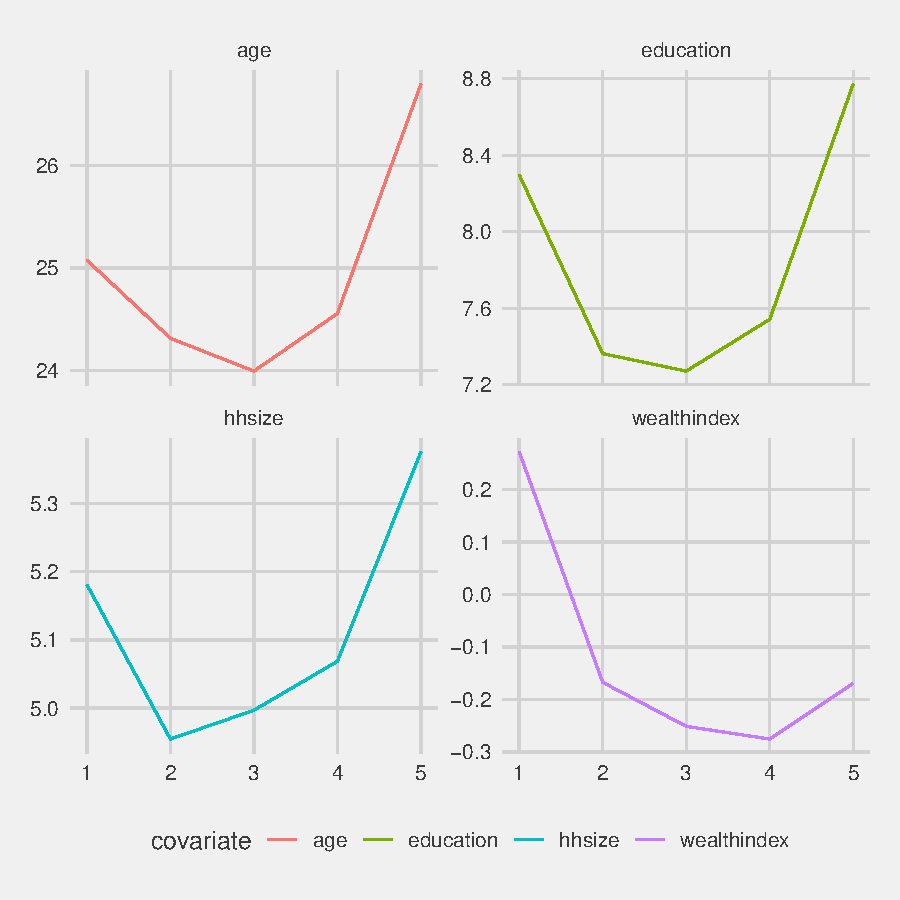
\includegraphics[width=.6\linewidth]{figure/rsa-ml-Rnwauto-report-1} 

}



\end{knitrout}

The R session information (including the OS info, R version and all
packages used):

\begin{knitrout}
\definecolor{shadecolor}{rgb}{0.969, 0.969, 0.969}\color{fgcolor}\begin{kframe}
\begin{alltt}
\hlkwd{sessionInfo}\hlstd{()}
\end{alltt}
\begin{verbatim}
## R version 4.0.3 (2020-10-10)
## Platform: x86_64-w64-mingw32/x64 (64-bit)
## Running under: Windows 10 x64 (build 19042)
## 
## Matrix products: default
## 
## Random number generation:
##  RNG:     Mersenne-Twister 
##  Normal:  Inversion 
##  Sample:  Rounding 
##  
## locale:
## [1] LC_COLLATE=English_United States.1252  LC_CTYPE=English_United States.1252   
## [3] LC_MONETARY=English_United States.1252 LC_NUMERIC=C                          
## [5] LC_TIME=English_United States.1252    
## 
## attached base packages:
## [1] stats     graphics  grDevices utils     datasets  methods   base     
## 
## other attached packages:
##  [1] ggthemes_4.2.0      randomForest_4.6-14 forcats_0.5.0       stringr_1.4.0      
##  [5] dplyr_1.0.2         purrr_0.3.4         readr_1.4.0         tidyr_1.1.2        
##  [9] tibble_3.0.4        ggplot2_3.3.2       tidyverse_1.3.0     haven_2.3.1        
## [13] knitr_1.30         
## 
## loaded via a namespace (and not attached):
##  [1] Rcpp_1.0.5        cellranger_1.1.0  pillar_1.4.7      compiler_4.0.3   
##  [5] dbplyr_2.0.0      highr_0.8         tools_4.0.3       digest_0.6.27    
##  [9] jsonlite_1.7.2    lubridate_1.7.9.2 evaluate_0.14     lifecycle_0.2.0  
## [13] gtable_0.3.0      pkgconfig_2.0.3   rlang_0.4.9       reprex_0.3.0     
## [17] cli_2.2.0         rstudioapi_0.13   DBI_1.1.0         curl_4.3         
## [21] xfun_0.19         withr_2.3.0       xml2_1.3.2        httr_1.4.2       
## [25] fs_1.5.0          generics_0.1.0    vctrs_0.3.5       hms_0.5.3        
## [29] grid_4.0.3        tidyselect_1.1.0  glue_1.4.2        R6_2.5.0         
## [33] fansi_0.4.1       readxl_1.3.1      farver_2.0.3      modelr_0.1.8     
## [37] magrittr_2.0.1    backports_1.2.0   scales_1.1.1      ellipsis_0.3.1   
## [41] rvest_0.3.6       assertthat_0.2.1  colorspace_2.0-0  labeling_0.4.2   
## [45] stringi_1.5.3     munsell_0.5.0     broom_0.7.3       crayon_1.3.4
\end{verbatim}
\begin{alltt}
\hlkwd{Sys.time}\hlstd{()}
\end{alltt}
\begin{verbatim}
## [1] "2021-01-13 02:55:30 GMT"
\end{verbatim}
\end{kframe}
\end{knitrout}


\end{document}
